%\exer{}
%\setcounter{numques}{0}

Un promeneur souhaite transporter dans son sac à dos le fruit de sa cueillette. La cueillette est belle, mais trop lourde pour être entièrement transportée dans le sac à dos. Des choix doivent être faits. Il faut que la masse totale des fruits choisis ne dépasse pas la capacité maximale du sac à dos.

Les fruits cueillis ont des valeurs différentes et le promeneur souhaite que son chargement soit de la plus grande valeur possible.

\begin{figure}[h]
\centering
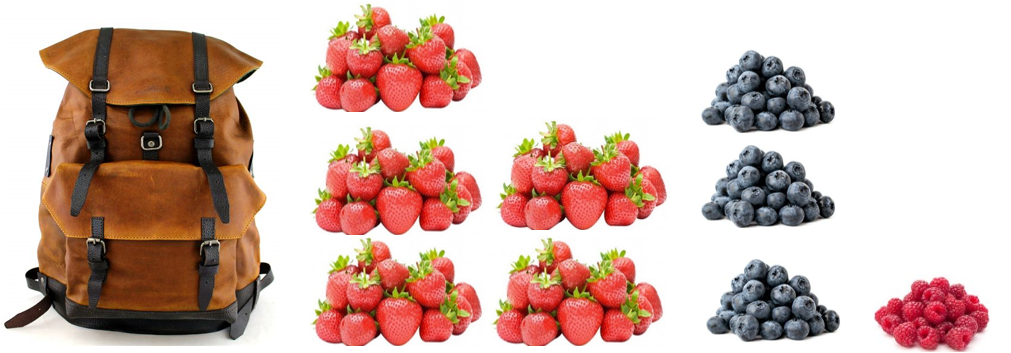
\includegraphics[width=.8\linewidth]{SacEtFruits.png}
\label{fig:SacEtFruits}
\end{figure}



\begin{table}[h]
\centering
\begin{tabular}{|l|c|c|}
\hline
Fruits cueillis	& Prix au kilo & Quantité ramassée\\
\hline
framboises& 24 €/kg  & 1 kg \\
myrtilles & 16 €/kg & 3 kg  \\
fraises & 6 €/kg & 5 kg \\
mures & 3 €/kg & 2 kg \\
\hline
\end{tabular}
\caption{}
\label{tab_fruit}
\end{table}

La capacité du sac à dos n’est que de \SI{5}{kg}.
On suppose que la masse d’un unique fruit est négligeable par rapport à la masse totale du sac en charge.

\subsection*{Présentation de l’algorithme et implémentation}
\label{sec:PrésentationDeLAlgorithmeEtImplémentation}

Le principe pour optimiser le chargement est de commencer par mettre dans le sac la quantité maximale de fruits les plus chers par unité de masse. S’il y a encore de la place dans le sac, on continue avec les fruits les plus chers par unité de masse parmi ceux restants... et ainsi de suite jusqu’à ce que le sac soit plein. Il est possible qu’on ne puisse prendre qu’une fraction de la quantité de fruits disponible, si la capacité maximale du sac est atteinte. %L’algorithme sera donc constitué d’une structure itérative, incluant une structure alternative.

%Dans \textbf{Algorithmes\_gloutons.py}, nous avons ébauché l’algorithme de résolution du problème et implémenté \texttt{cueillette} par la liste des fruits \textbf{triée} par prix au kilo décroissant.\\
Un fruit est représenté par une liste \texttt{fruit=[prix au kilo,nom,quantité ramassée]} :

\texttt{cueillette = [[24,"framboises",1], [16,"myrtilles",3], [6,"fraises",5], [3,"mures",2]]}


\question{Implémenter la fonction \texttt{sac\_a\_dos(L:list, capacite:int)} qui prend en argument une liste de listes \texttt{L} modélisant la cueillette et la capacité du sac à dos, et appliquant la méthode décrite précédemment. Cette fonction renvoie :}
\textit{\begin{itemize}
\item une liste de listes des fruits contenus dans le sac à dos avec leur masse correspondante de façon à avoir le chargement de valeur maximale ;
\item la valeur du chargement.
\end{itemize}}

La liste \texttt{cueillette} ne doit pas être modifiée. Vous pourrez si nécessaire utiliser une copie de la liste  \texttt{cueillette} que vous pourrez modifier. La copie de liste de listes se fait avec les instructions :
\begin{lstlisting}
import copy # au début de votre script
L=copy.deepcopy(votreListe) # quand cela est nécessaire
\end{lstlisting}


\question{Exécuter votre programme et vérifier le résultat.}


Une variante de ce problème ne trouve pas de solution optimale par la méthode gloutonne. Nous l’étudions ci-après.

\subsection*{Version non fractionnaire du problème du sac à dos}
\label{sec:VersionNonFractionnaireDuProblèmeDuSacÀDos}

On suppose maintenant que les éléments à transporter ne sont pas fractionnables. Les fruits parmi lesquels choisir sont présentés dans le tableau \ref{tab_fruit2}.


\begin{table}[h]
	\centering
		\begin{tabular}{|l|c|c|c|}
\hline
Fruits  & Prix au kilo & Masse d’un fruit & Quantité disponible\\
\hline
melon de cavaillon & 3 €/kg & 1 kg & 1\\
melon jaune  & 2.5 €/kg & 2 kg & 1\\
pastèque & 2 €/kg & 3 kg & 1 \\

\hline
		\end{tabular}
		\caption{}
	\label{tab_fruit2}
\end{table}

Cet ensemble de fruits est modélisé par :
\begin{itemize}
\item un fruit non fractionnable est représenté par une liste \texttt{[prix au kilo,nom,masse,quantité disponible]};
\item une liste de listes \texttt{fruitsDisponibles = [[3,"melon de cavaillon",1,1], [2.5,"melon jaune",2,1, 2,"pastèque",3,1]]}.
\end{itemize}



L’objectif est toujours de placer dans le sac à dos le chargement de valeur maximale, de masse totale inférieure à 5kg. Par contre, les éléments n’étant fractionnables, il est possible que les choix successifs mène à un chargement qui ne remplit pas complètement le sac à dos.

On se propose de tester la méthode gloutonne pour cette nouvelle formulation. 

\question{En adaptant la fonction \texttt{sac\_a\_dos(L , capacite)} que vous renommerez \texttt{sac\_a\_dos\_V2(L , capacite)}, adapter la fonction de sorte qu’elle applique la méthode gloutonne à la version non fractionnaire du problème. %Pour cela, il faut :
%\begin{itemize}
%	\item {commenter la structure conditionnelle permettant de continuer à remplir le sac si sa capacité restante est inférieure à la masse du i-ème fruit,}
%	\item {adapter la condition de la structure itérative de sorte à ne continuer à remplir le sac que si la capacité le permet.}
%\end{itemize}
Exécuter la fonction en utilisant la liste \texttt{fruitsDisponibles}.}

\question{Le résultat obtenu est-il optimal ? Comparer avec la solution S = [[2.5,"melon jaune",2,1], [2,"pastèque",3,1]]. Quelle est la solution dont la valeur est maximale ?}



